\documentclass[11pt,dvipdfmx,a4paper]{jsarticle}

\usepackage{amsmath,amssymb}
\usepackage{bm}
\usepackage[dvipdfmx]{graphicx}
\usepackage{physics} % http://mirrors.ibiblio.org/CTAN/macros/latex/contrib/physics/physics.pdf
\usepackage{siunitx} %SI単位を楽に出力
\usepackage{mathtools} %環境の追加
% \usepackage{circuitikz} %電気回路をtex中で書く
% \usepackage{caption} %番号なしキャプションを書く
% \usepackage{cancel} %式中に斜線を入れる
% \usepackage{tensor} %テンソルの添え字を書く
% \usepackage{tikz} %図を書く
% \usepackage{ascmac} %四角い枠の中に文章を書く
% \usepackage{float} %figureで[hbp]オプションを使う
% \usepackage{hyperref}  \usepackage{pxjahyper} %ハイパーリンクをつかう
% \usepackage{tablefootnote} %表中に注釈をいれる
% \usepackage[thicklines]{cancel} %数式中の取り消し線
\usepackage[version=4]{mhchem} %化学式の入力
\usepackage{pdfpages}
% \usepackage{wrapfig} %文章の回り込み
\usepackage[subrefformat=parens]{subcaption} %(a)図のようにすることができるやつ
\usepackage{here}
\usepackage{mathrsfs} % TODO テンプレートに追加
\usepackage{url} % TODO テンプレートに追加
\usepackage[margin=15mm]{geometry} %余白の削除

\graphicspath{{./image/}}

\begin{document}

%出力したpdfを表紙にするとき
% \includepdf[pages=1,noautoscale=false]{cover.pdf}
% \newpage

%texで表紙を書くとき
\quad\\[35mm]
\centerline{\Huge{\textsf{第 4 回}}}
\quad\\[5mm]
\centerline{\Huge{\textsf{応 用 物 理 学 実 験}}}
\quad\\[5mm]
\begin{table}[h]
	\centering
	\begin{tabular}{| c | c |}
		\hline
		\Huge\textsf{{題目}} & \Huge{\textsf{電気伝導度の温度依存性}} \rule[-5mm]{0mm}{15mm} \\
		\hline
	\end{tabular}
\end{table}
\quad\\[10mm]
\begin{table}[h]
	\centering
	\begin{tabular}{l l}
		\hline
		\LARGE{\textsf{氏\qquad 名}} & \LARGE{\textsf{: 西原 翔}} \rule[0mm]{0mm}{6mm} \\
		\hline
		\LARGE{\textsf{学  籍  番  号}} & \LARGE{\textsf{: 1522068}} \rule[0mm]{0mm}{6mm} \\
		\LARGE{\textsf{学部学科学年}} & \LARGE{\textsf{: 理学部第一部応用物理学科3年}}\\
		\hline
	\end{tabular}
\end{table}
\quad\\[10mm]
\centerline{\LARGE{\textsf{共同実験者:1522064 中井空弥}}}\\[2mm]
\centerline{\LARGE{\textsf{\qquad\qquad\quad\;\;1522091 宮田祟杜}}}\\[2mm]
\centerline{\LARGE{\textsf{\qquad\qquad\quad\;\;1522095 村山涼矢}}}\\[2mm]
\centerline{\LARGE{\textsf{\qquad\qquad\quad\;\;1522B02 中村洸太}}}\\[2mm]
\quad\\[10mm]
\centerline{\LARGE{\textsf{提出年月日:2024年06月27日}}}\\[2mm]
\centerline{\LARGE{\textsf{実験実施日:2024年06月14日}}}\\[2mm]
\centerline{\LARGE{\textsf{\qquad\qquad\quad\;2024年06月21日}}}
\quad\\[10mm]
\centerline{\LARGE{\textsf{東 京 理 科 大 学 理 学 部 第 1 部}}}\\[2mm]
\centerline{\LARGE{\textsf{応 用 物 理 学 教 室}}}

\thispagestyle{empty}
\clearpage
\addtocounter{page}{-1}
\newpage

% \twocolumn
\section{目的}

\section{原理}
\subsection{ドルーデモデル}
量子論以前の1900年頃、
ドルーデは電気伝導について古典的なモデルを立てて議論した。
電子を外部電場\(\mathscr{E}\)のなかの理想気体と考え、
古典的な運動方程式で記述する。
電子気体はイオンや欠陥によって散乱されるものとして、
運動方程式を立てると。
\begin{align}
    m\dot{v} + \frac{m}{\tau}v = -e\mathscr{E} % \tag{9.42}
\end{align}
このときの\(v_D\)はドリフト速度というもので電子の速度から
電場のない熱平衡状態における電子の速度\(v_{\text{therm}}\)
を用いて
\begin{align}
    v_D= v-v_{\text{therm}}
\end{align}
と表されるものである。
電場がないときこの古典的な運動方程式の解としては
\begin{align}
    v = v_{\text{therm}}\qty(1-e^{-t/\tau})
\end{align}
である。
電場があるときには解は
\begin{align}
    v = -\frac{e\mathscr{E}\tau}{m}\qty(1-\exp\frac{-t}{\tau})
\end{align}
となっているので\(\tau\)は平衡状態に達するまでの緩和時間。
ドリフト速度は
\begin{align}
    v_D=-\frac{e\tau}{m}\mathscr{E} % \tag{9.43}
\end{align}
となる。
これより電場方向の電流密度は熱平衡状態では電流が流れてないのでドリフト速度を用いて
\begin{align}
    j = -env_D = ne\mu\mathscr{E} = \frac{e^2\tau n}{m}\mathscr{E} % \tag{9.44}
\end{align}
このとき\(n\)は自由電子の体積密度、
移動度\(\mu\)は電場をかけたときのドリフト速度の比例定数。
これより伝導度は
\begin{align}
    \sigma = \frac{j}{\mathscr{E}} = \frac{e^2n\tau}{m} % \tag{9.45}
\end{align}
と表される。
この式より、電気伝導度は電流のキャリア濃度に比例することがわかる。

\subsection{半導体への不純物ドーピング}
半導体に電子をドープしたときのバンドの様子を考える。
ここの記述は『初歩から学ぶ固体物理学\cite{Yaguchi_2017}』を参考にした。
バンドモデルでは一電子近似の元で考える。
周期ポテンシャルのもとのシュレーディンガー方程式は
周期ポテンシャルを \(V(r)\), ドープした原子によるポテンシャルを \(\hat{H}'(r)\) として
\begin{equation}
	\qty(-\frac{\hat{p}^2}{2m}+V+H')\psi = E \psi
\end{equation}
となる。
\(H'(r)\) によるポテンシャル変化は周期ポテンシャルに比べ変化はゆっくりしている。
こうしたときには周期ポテンシャルによる波動関数への寄与は質量の部分に取り込むことができる。
今回使う半導体は \ce{n-Ge} であり伝導体の最下部は \(\Gamma\) 点にある。

なので
\begin{equation}
	\qty(-\frac{\hbar^2}{2m^*}+\hat{H}'(r))F(r) = (E-E_c)F(r)
\end{equation}
とできる。ドープした原子は陽イオンとみなせるため
\begin{equation}
	\hat{H}'(r) = -\frac{e^2}{4\pi\varepsilon r}
\end{equation}
とできる。するとこれは水素原子と同じ問題になるため、この固有値方程式の固有値は
\begin{align}
	E-E_c &= -\frac{m^*}{2}\qty(\frac{e^2}{4\pi\hbar\varepsilon})^2\frac{1}{n^2}\\
    E &= E_c -\qty(\frac{m^*}{m(\varepsilon/\varepsilon_0)^2})\frac{1}{n^2}\times\frac{m}{2\hbar^2}\qty(\frac{e^2}{4\pi \hbar\varepsilon_0})
\end{align}
というように不純物により新しい準位ができていることがわかる。
これをドナー準位という。
この式に\ce{AsGa}の各物理量の値を入れていくと
\begin{equation}
    E-E_c = 6\,\si{meV}
\end{equation}
というようになる。
100 K の温度によるゆらぎ\(k_B T\) はおおよそ 8 meV であるため、
ドナー準位は温度による影響を考えなければならないことがわかる。

\subsection*{4端子法}
オームの法則の式を変形して測定しやすい形にすると
\begin{equation}
  \sigma = \frac{J}{E} = \frac{I}{S} \times \frac{l}{V} = \frac{l}{SR}
\end{equation}
となる。つまり試料の断面積・長さを計測したのち、ある電流値を流したときの電圧差を測定すればよいというのがわかる。
この実験系を素直に組むと次の図2のようになる。この測定の仕方を2端子法という。
\begin{figure}[h]
  \centering
  \begin{minipage}[t]{0.49\columnwidth}
    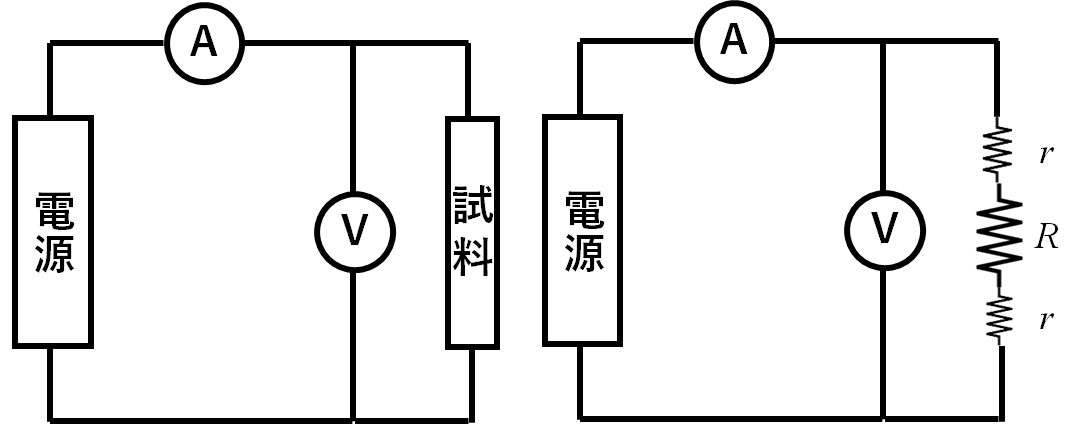
\includegraphics[width=\columnwidth]{/fig/fig2.png}
    \subcaption{2端子法}
  \end{minipage}
  \begin{minipage}[t]{0.49\columnwidth}
    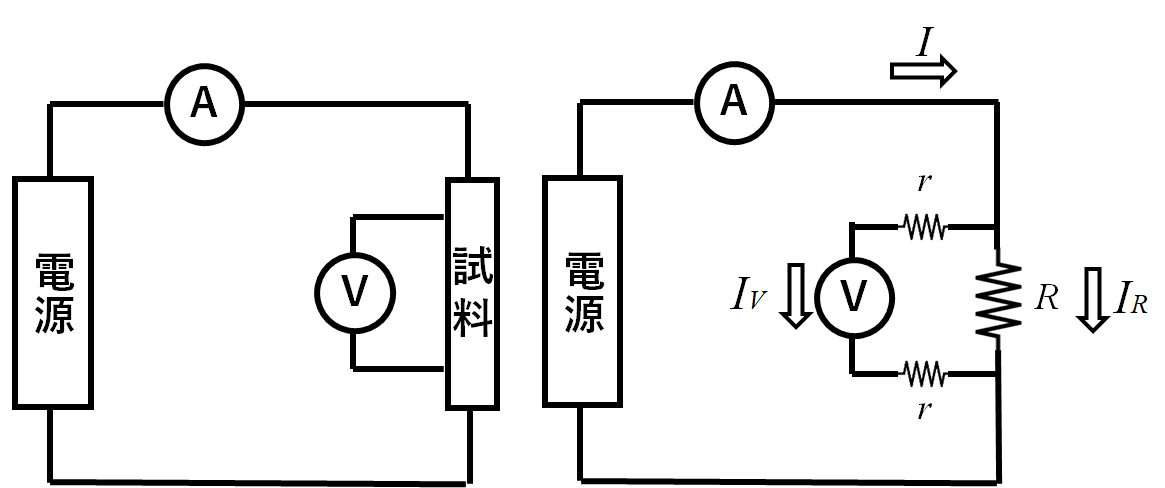
\includegraphics[width=\columnwidth]{/fig/fig3.png}
    \subcaption{4端子法}
  \end{minipage}
  \caption{回路図。接触抵抗・導線の抵抗をまとめて$r$電流を$I_R$、
  試料の抵抗を$R$電流を$I_V$、総電流を$I$、とおいている}
\end{figure}\\
普段の測定の場合接触抵抗\(r\)は十分小さいと考えられるため、
接触抵抗の存在を無視して試料の抵抗値を電流・電圧計から読み取った値からそのまま計算することで
試料の抵抗値を計測できる。これは回路方程式で表すと
\begin{equation}
  V=I(R+2r)=IR(1+\frac{2r}{R}) \stackrel{r<<R}{=} IR
\end{equation}
しかし試料の抵抗値がこの接触抵抗と同じほどの大きさの場合にはこのように考えることはできず
計測の意味がなくなる。これを解消するのに次の図3で示されるような4端子法という方法で行う。
試料にかかる電圧と接続抵抗・電圧計にかかる電圧に関しての等式は電圧計の内部抵抗を$R_m$とおくと
\begin{align}
  I_R R &= I_V (R_m + 2r)\\
  I_V &= \frac{IR}{R_m + 2r + R}
\end{align}
これより電圧計に表示される値は
\begin{equation}
  V=\frac{R_m}{R_m+ +2r + R} IR \stackrel{R_m>>r,R}{=} IR
\end{equation}
よって4端子法をつかうことで接続抵抗と試料の抵抗が同じほどの抵抗値を持っていたとしても、
電流計・電圧計から読み取った値を素直に使っても正確な試料の抵抗値が求まることがわかる。

\section{実験}
金属、p 型半導体、超伝導体の電気伝導度の温度依存性を調べるため、
金属として \ce{Pt}, p 型半導体として \ce{n-Ge}, 超伝導体として \ce{Nb} を試料とし、
断熱して温度を下げやすくするため、真空中に端子づけした試料をいれ、
四端子法と二端子法にて185 K から \ce{Nb} が超伝導相へと相転移する 8 K 程度まて
電気伝導度を測定した。その際に使った真空ポンプの様子は図\ref{pic:measure_system},
この系の電気回路は図\ref{fig:circuit_system}の通りになっている。

\begin{figure}[h]
	\centering
	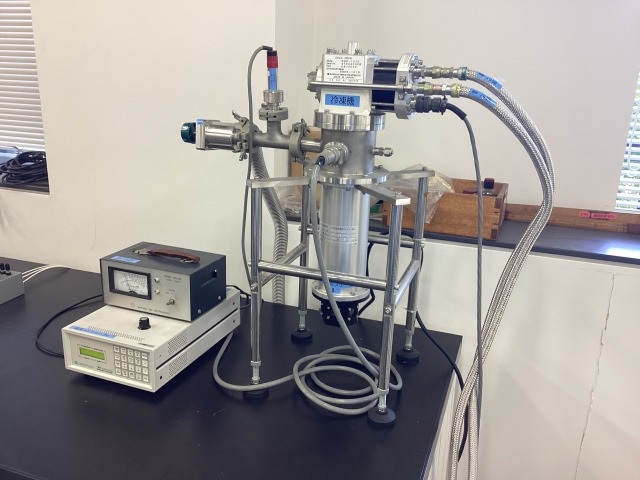
\includegraphics[width=0.5\columnwidth]{pic/01.jpg}
	\caption{
		電気伝導度を真空中で測定する装置。
		上部から出ている管は試料室の温度を下げるための冷媒が流れている。
		下部には今回測定する 3 つの試料、\ce{Pt}, \ce{n-Ge}, \ce{Nb} が端子づけされた状態で入っている。
        これの温度や電流電圧値はデジタルマルチメータで測定する。
		左には真空へと排気するポンプへつながる管がつながっている。
	}
	\label{pic:measure_system}
\end{figure}
\begin{figure}[h]
	\centering
	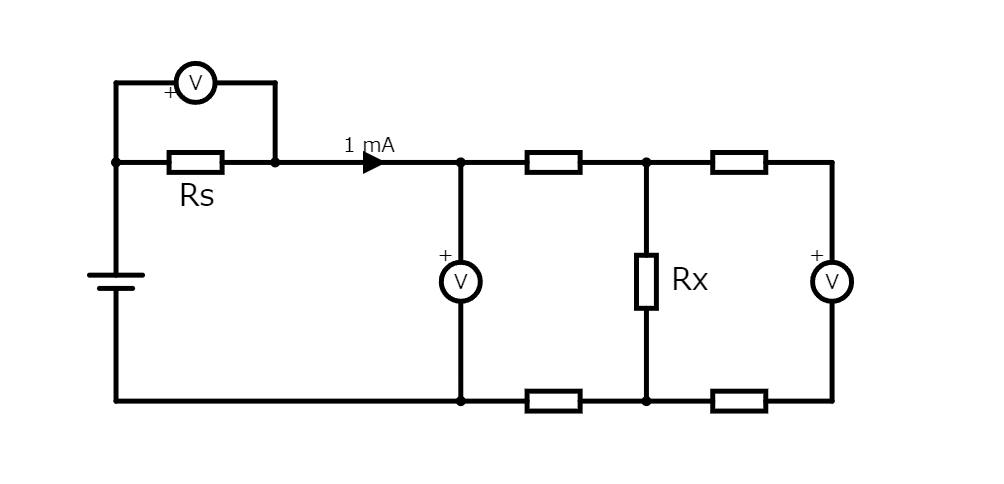
\includegraphics[width=0.75\columnwidth]{fig/fig4.png}
	\caption{測定する系の電気回路図。
    直流電源によって抵抗値\(R_x\)の抵抗に電圧をかける。
    \(R_s\)は標準抵抗で電流値を測定するためのもの。
    残りの抵抗は配線抵抗と接触抵抗をまとめたもの。
    左の電圧計は2端子法、右の電圧計は4端子法での測定用のもの。
    黒い三角は電流計。
	}
	\label{fig:circuit_system}
\end{figure}

\clearpage
\section{結果}
\ce{n-Ge} の電気伝導度を二端子法と四端子法で測定した結果をアレニウスプロットすると図\ref{graph:n-Ge_ex}のようになった。
4端子法の結果をみると、
始め高温では電気伝導度が増えていく出払い領域が見られる。
30 K 以下の不純物領域では電気伝導度は減少していき、直線近似できる部分が2箇所あるのがわかる。

各温度における \ce{Pt} と \ce{Nb} の抵抗率の測定結果を残留抵抗による寄与を取り除いて、
デバイ温度における抵抗率で規格化すると、
図\ref{graph:Pt_Nb_ex}のようになった。
\ce{Pt} の結果はグリュナイゼン\cite{Grueneisen}による抵抗率の温度依存性の式に
とてもよく一致している。
一方 \ce{Nb} は 8.1 K において抵抗率の値が3桁減少する振る舞いが見られた。
これは超伝導相への転移によるものと思われる。
超伝導による転移の寄与を取り除いた結果を見ると
おおよそグリュナイゼンによる式と同じような振る舞いをするようになった。

また、今回測定した試料の特徴的な値をまとめると表\ref{table:parameter}のようになった。
\begin{figure}[h]
    \centering
    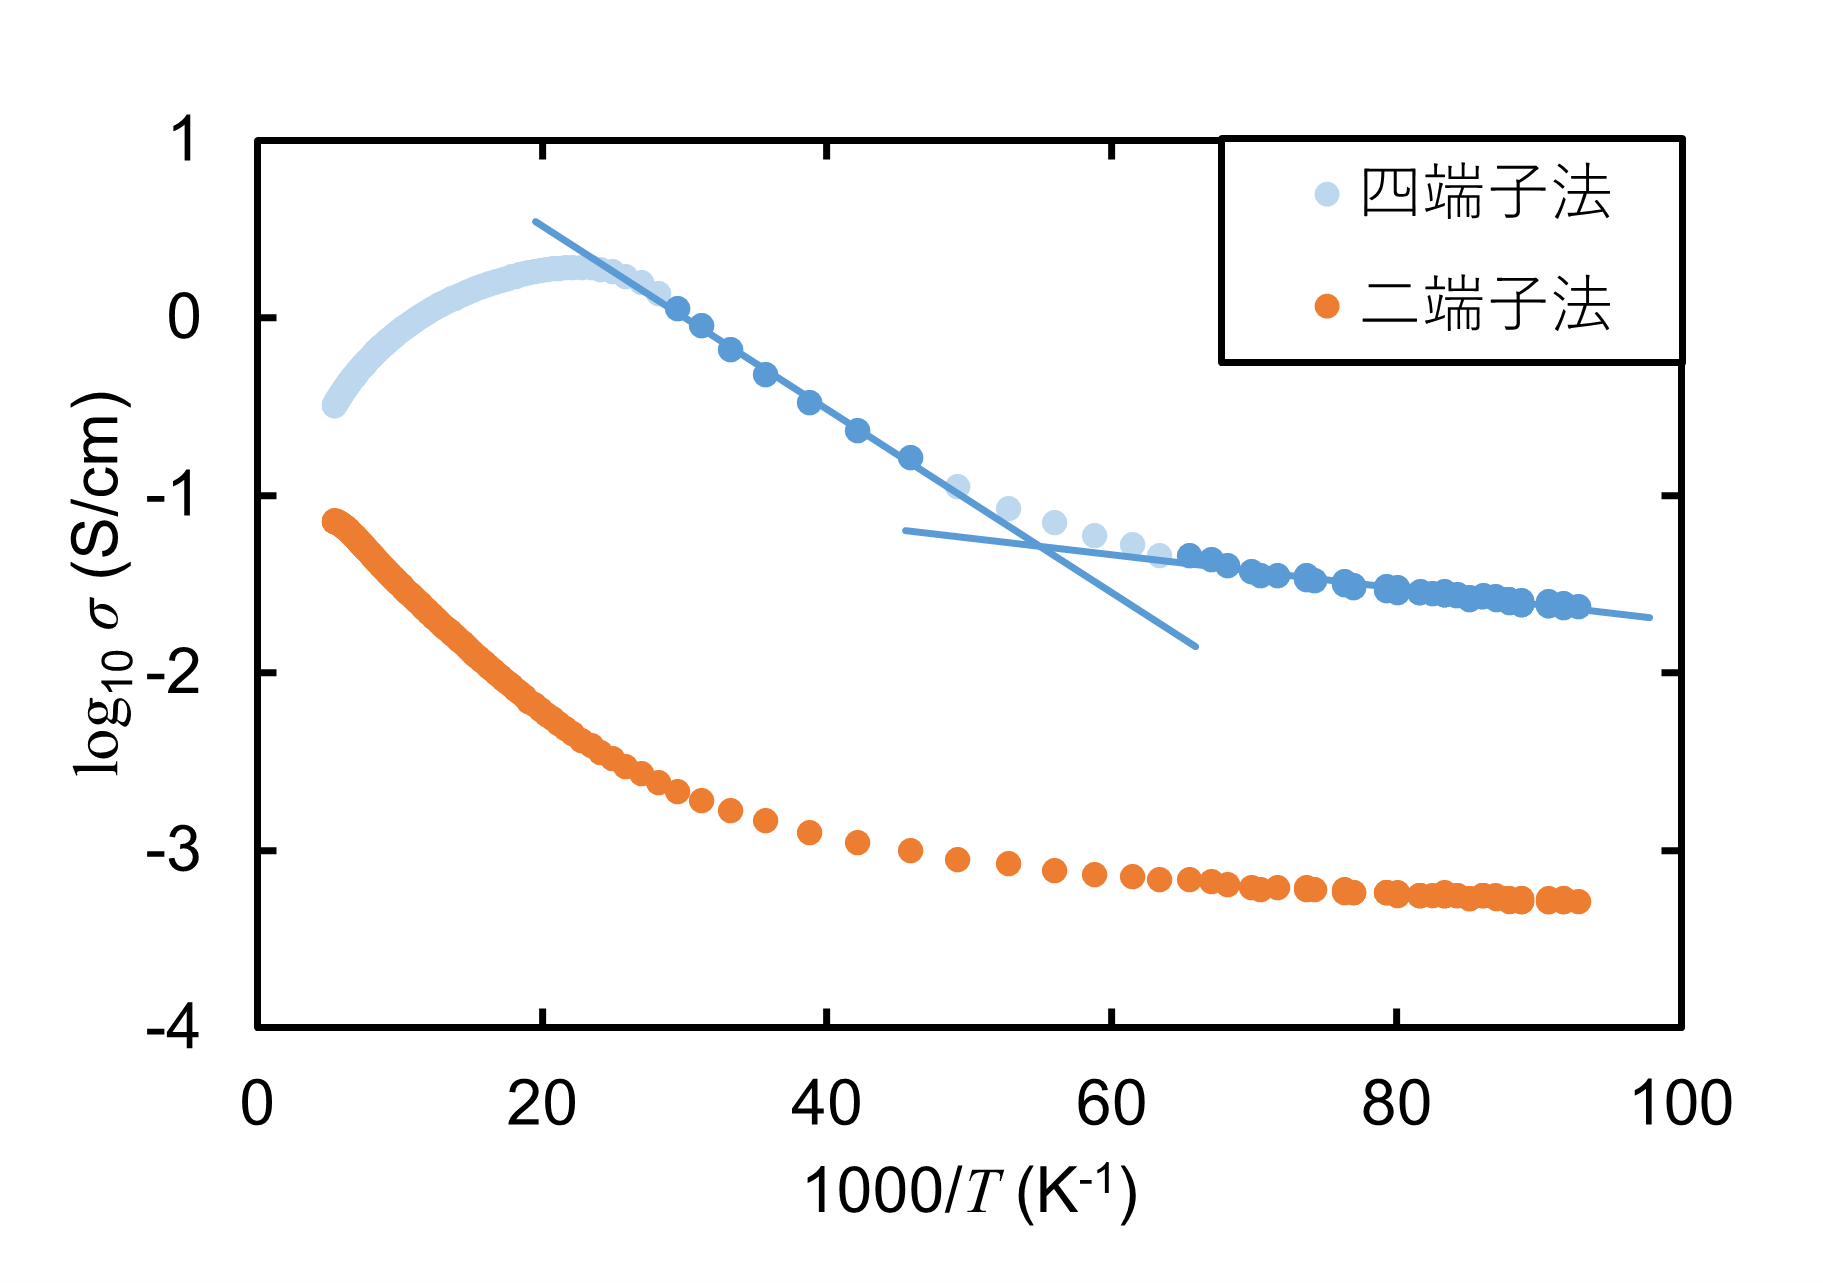
\includegraphics[width=0.5\columnwidth]{/graph/graph01.png}
    \caption{n-Ge の電気伝導度の温度依存性を2端子法と4端子法で測定したものをアレニウスプロットしたもの。
    4端子法では左から出払い領域、と直線状になっている不純物領域が二つあるのがわかる。
    2端子法の結果を見ると電気抵抗が4端子法に比べ高く、意図しない抵抗の温度特性を測定していることになっているのがわかる。}
    \label{graph:n-Ge_ex}
\end{figure}

\begin{figure}[h]
    \centering
    \begin{minipage}[t]{0.48\columnwidth}
        \centering
        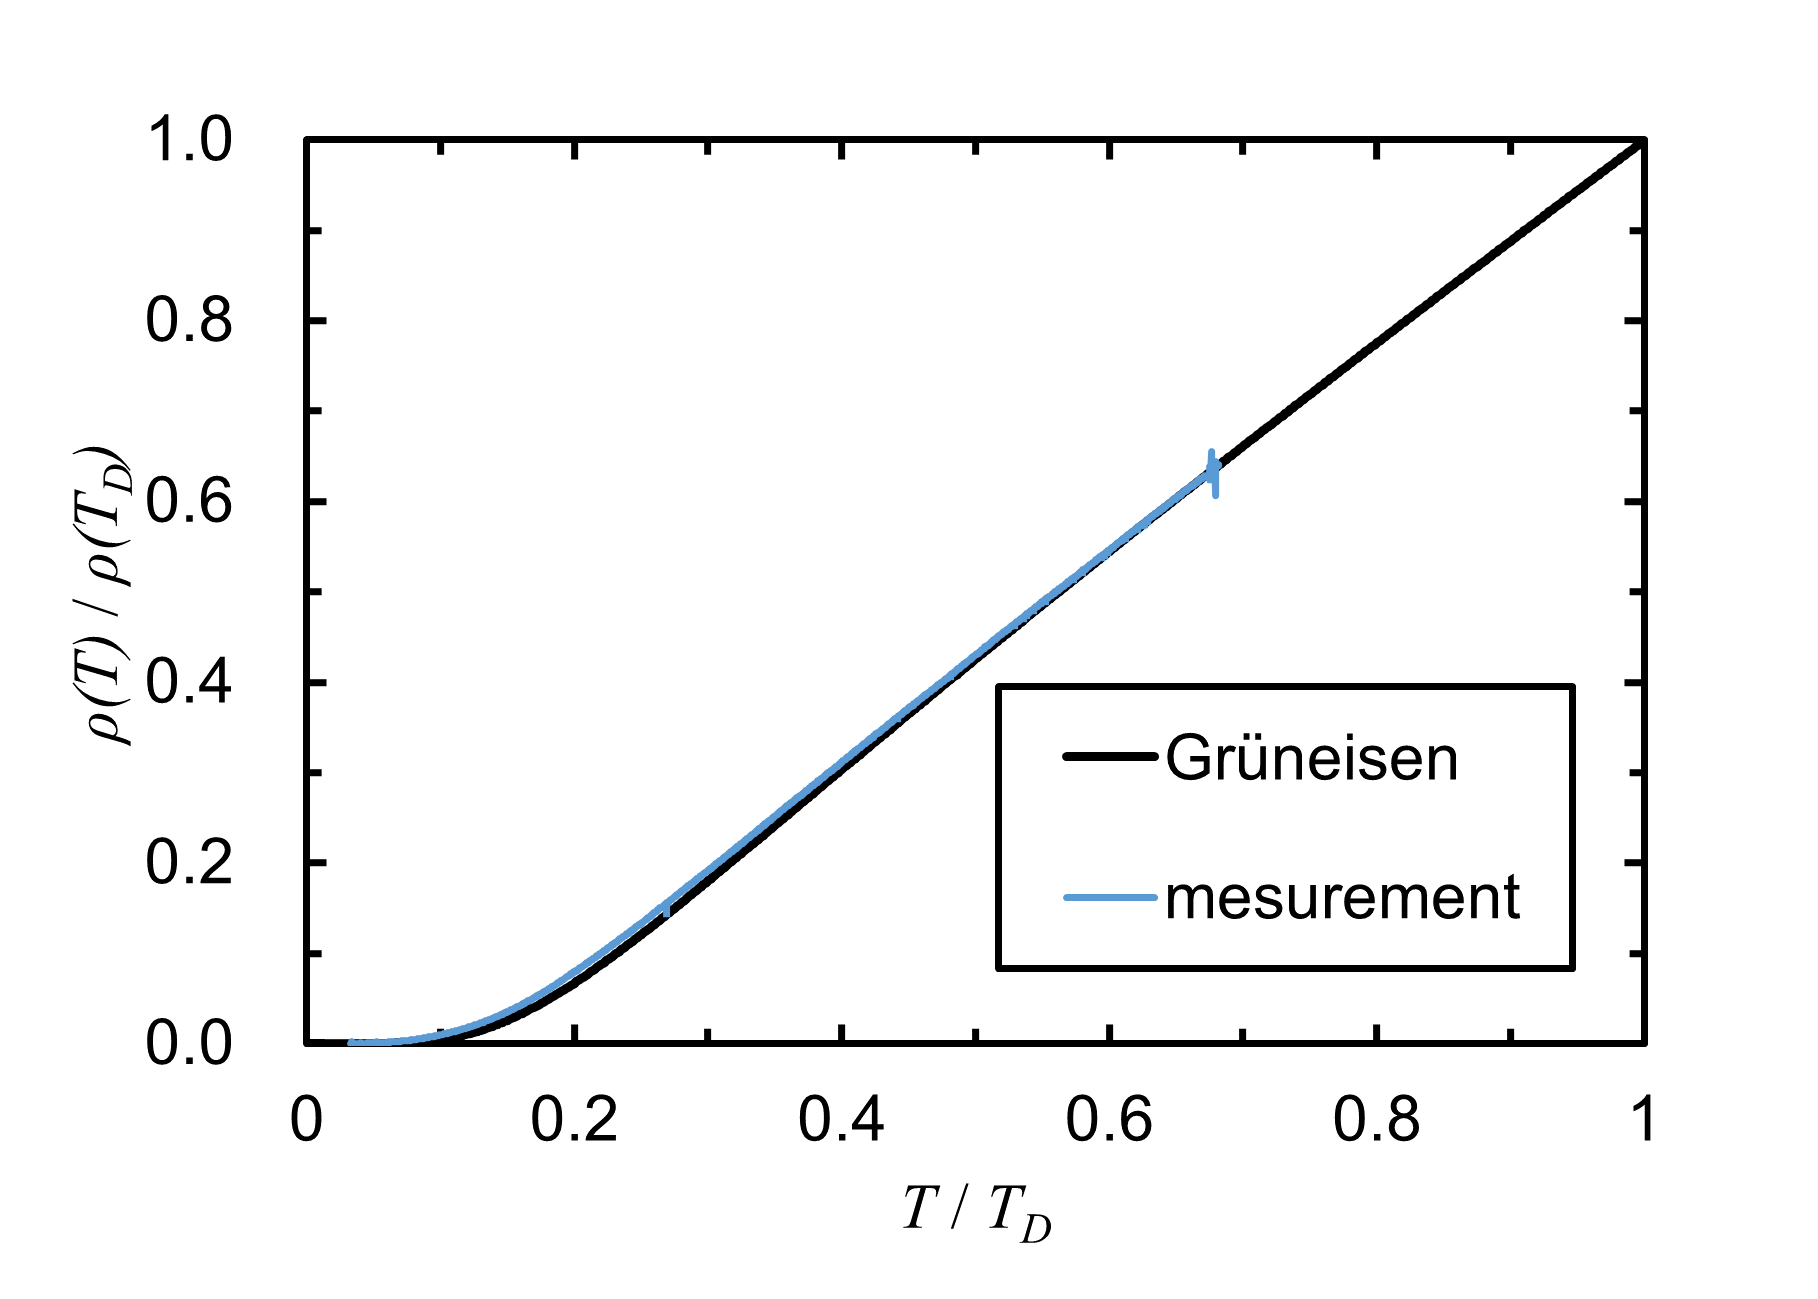
\includegraphics[width=\columnwidth]{graph/graph02.png}
        \subcaption{\ce{Pt}の抵抗率の測定結果。残留抵抗を取り除いてある。}
    \end{minipage}
    \hfill
    \begin{minipage}[t]{0.48\columnwidth}
        \centering
        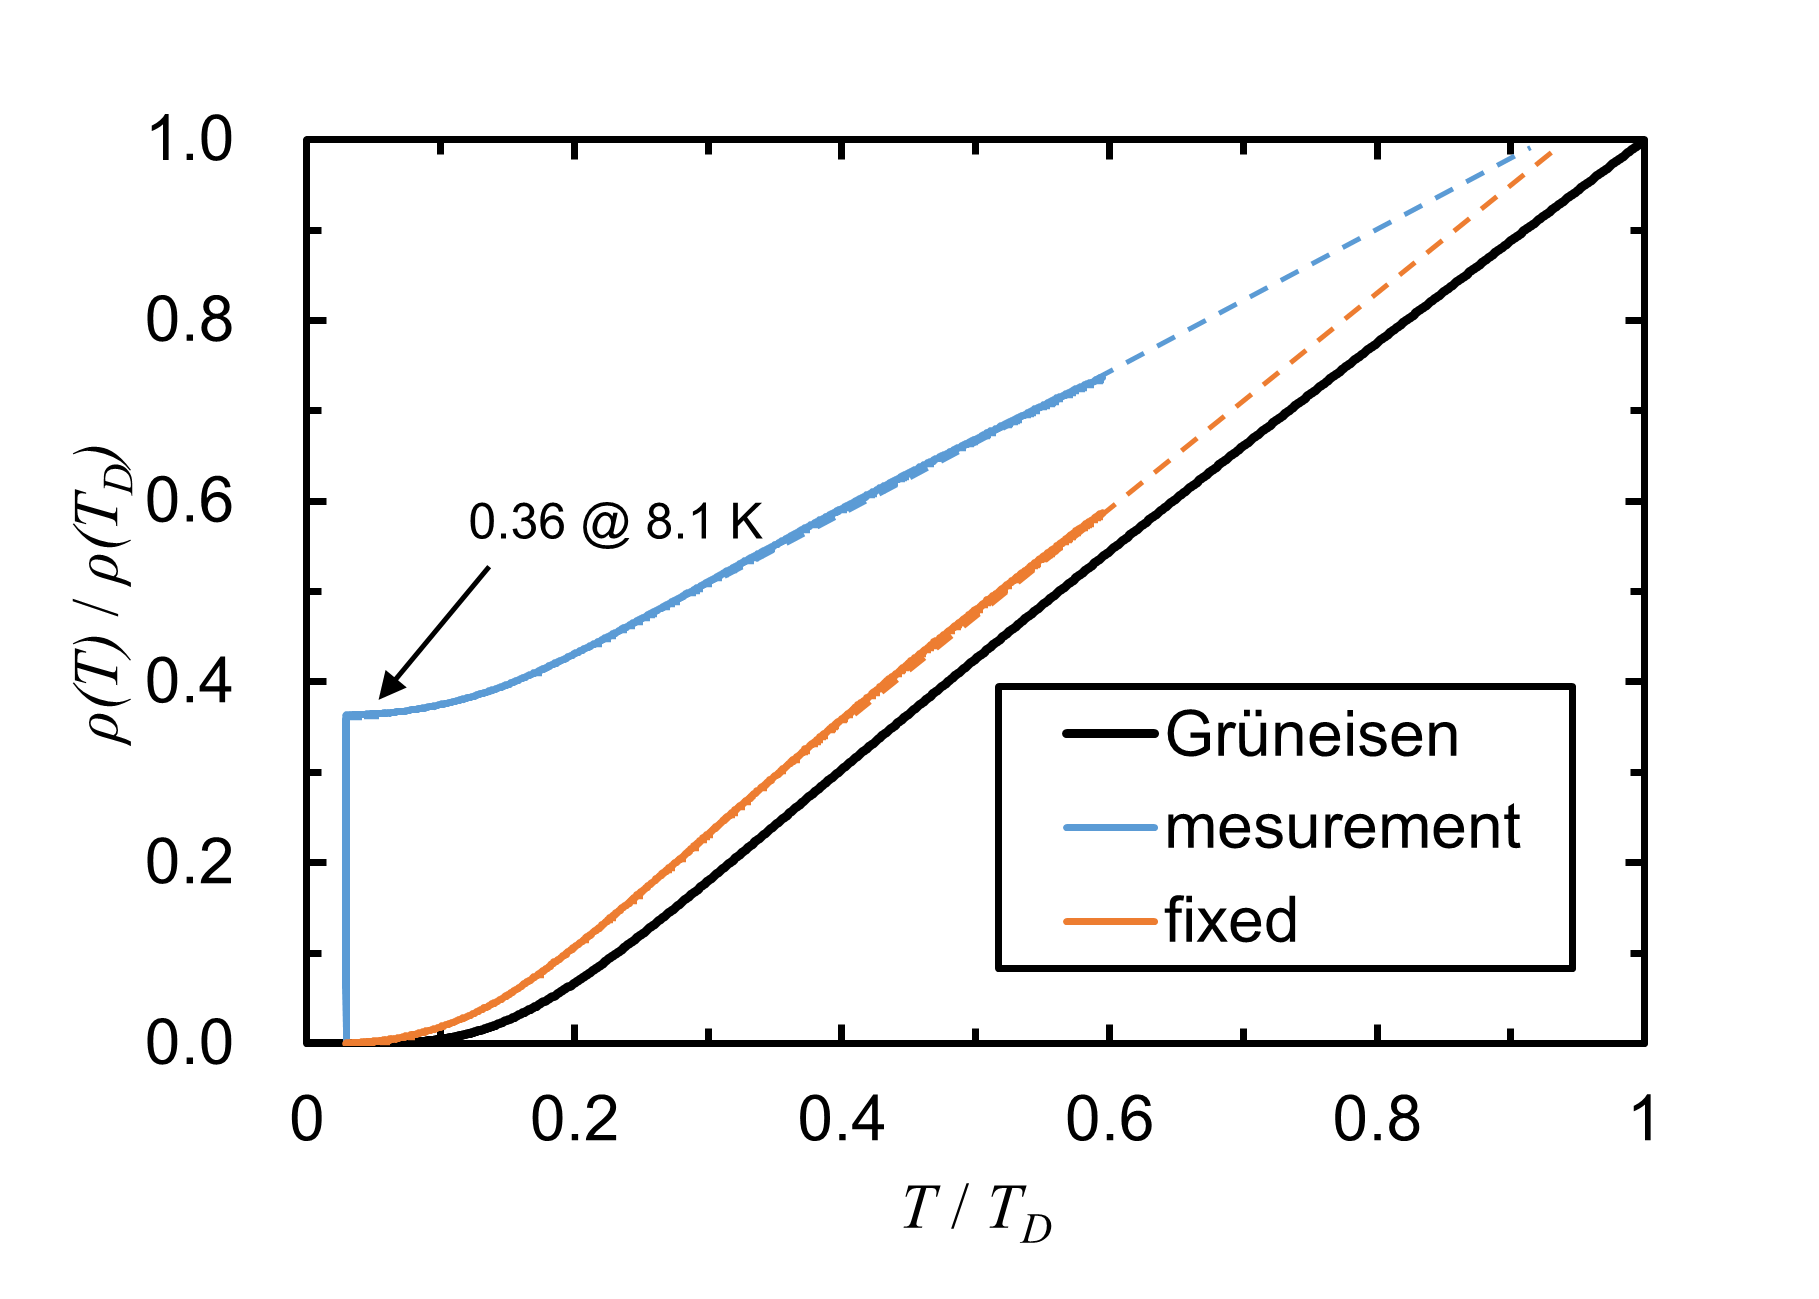
\includegraphics[width=\columnwidth]{graph/graph03.png} % TODO legend が変
        \subcaption{\ce{Nb}の抵抗率の測定結果}
    \end{minipage}
    \caption{金属と超伝導体の電気抵抗率の測定結果。
    デバイ温度とそこにおける抵抗率で規格化してある。
    測定結果とグリュナイゼンの式の結果。
    超伝導転移する\ce{Nb}は抵抗率をプロットする際に、
    測定値を規格化したものと、超伝導転移温度における抵抗率の寄与を取り除いたものをプロットした。
    また、\ce{Nb} には測定していない温度における抵抗率を外挿した。}
    \label{graph:Pt_Nb_ex}
\end{figure}
\begin{table}[h]
    \centering
    \caption{\ce{n-Ge}, \ce{Pt}, \ce{Nb} の各パラメータ。ただし、残留抵抗抵抗比はデバイ温度との比になっている。}
    \label{table:parameter}
    \begin{tabular}[pos]{lccc}
        \hline
         & \ce{n-Ge} & \ce{Pt} & \ce{Nb}\\
         \hline
         デバイ温度\(T_D\) (K) & 374 & 240 & 275\\
         \(R(T_D)\) (\si{\ohm}) & - & 863 & 6.63\\
         残留抵抗 (\si{\ohm}) & 42.3 & 8.65 & - \\
         残留抵抗比 & - & 99.8 & -\\
         超伝導転移温度(K) & - & - & 8.1 \\
         \hline
    \end{tabular}
\end{table}

\section{課題}
\subsection*{課題1}
金属のフェルミ準位はバンドの中を通るのに対し、
半導体はバンドの中を通らない。
金属と半導体を接合する際にはフェルミ準位が同じになるように
バンドは接合される。
すると金属と半導体の伝導電子のバンドに差が大きくできてしまう。
これによる障壁は半導体のバンドギャップ\(E_g\)程度のオーダーであるため、
電圧に直すと 0.5 V 程度の電圧が接合面にかかっているといえる。
これより、接触抵抗が想定されるものよりも大きくなる。

\subsection*{課題2}
図\ref{graph:n-Ge_ex}を見ると 30 K より高温では、
ドナー準位からキャリアが出ていく、出払い領域になっているとわかる。
低温から高温へとグラフを見ていったとき 30 K で電気伝導度の上昇が終わる。
これはつまり、30 K 程度であればドナー準位から伝導帯の間のエネルギーギャップは
熱ゆらぎで十分飛び越せることを意味する。
熱ゆらぎのオーダーは\(\sim k_BT\)であるので、ドナー準位と伝導バンドのエネルギーギャップは
\begin{equation}
    E_c - E \sim k_B T = \text{ meV}
\end{equation}
オーダーであると推定できる。

\subsection*{課題3}
電気伝導度はキャリア密度に比例し、
またキャリア密度はグランドカノニカル分布から計算すると低温では
\begin{equation}
    n \propto \exp(-\frac{E_d}{2k_bT})
\end{equation}
になる。
つまり電気伝導度の対数を取ったものは
\begin{equation}
    \ln \sigma = -\frac{E_d}{2000k_b} \frac{1000}{T} + \text{const.}.
\end{equation}
これよりアレニウスプロットで電気伝導度が下がる不純物領域の傾きを見ることで
ドナー準位と伝導体とのエネルギー差を求めることができる。
今回の測定結果では直線とみなせる部分が2箇所あるのでそこの傾きでエネルギー差を求めると
\begin{equation}
    E_d = 20 \text{ meV},\quad 1.57 \text{ meV}
\end{equation}
となった。

\subsection*{課題4}
この測定結果では不純物領域のアレニウスプロットの傾きが2通りあるのがわかる。
これはつまり電気伝導度を単にキャリア密度に比例するものだと考えてはならないことを意味する。
ドゥルーデモデルでは
\begin{equation}
    \sigma = \frac{ne^{*2}\tau}{m^*}
\end{equation}
であった。
今回使った\ce{Ge}半導体は\(\Gamma\)点からの直接遷移型の半導体であり、
有効質量となる\(\Gamma\)点でのバンドの曲率は温度に依存しない。
また、有効電荷も変わらない。
では電子の散乱を表す\(\tau\)の項がどのように効くか考える。
バンド電子が散乱するのはフォノン、不純物、格子欠陥、
といったようにさまざまな要因が考えられる。
フォノンによる散乱というのは要するに、原子核の振動が電子と相互作用することである。
低温になると格子振動の振幅が小さくなるため、電子と相互作用しなくなっていく。
そのため、フォノンとの散乱が原因ではない。

この原因は不純物や欠陥などにより結晶性が悪くなり、
伝導電子がバンド電子と局在電子の2種類あることに由来する。
結晶性が悪くなると、エネルギー準位は禁制帯をもったキレイなバンドにはならず、
禁制帯のなかに離散的な準位をとるようになる。
温度を下げていったときに 30 K 付近の伝導を担っているのはアクセプタ準位からのバンド電子
であるが、さらに下がっていくとこれらの電子も励起できなくなる。
そういったときに伝導を担うのが局在電子になる。
この局在電子はホッピングして伝導していき、そのホッピングする距離は \(10^{-6}\) m 程度になる\cite{ibach-luth}。

\subsection*{課題5}
\ce{Pt} の抵抗率はグリュナイゼンの式とよく合った一方、
\ce{Nb} の抵抗率はそのままではまったく合わなかった。
超伝導臨界温度\(T_c\)における抵抗の値を引いたもの、
つまり
\begin{equation}
    \frac{\rho(T)-\rho(T_c)}{\rho(T_d)-\rho(T_c)}
\end{equation}
としてプロットするとグリュナイゼンの式とおおよそおなじような振る舞いをするようになった。
ただそれでも式とのずれというのは確認できた。
具体的には、全体的に抵抗率が高い点や、
抵抗率の値を外挿した際、\((1,\,1)\)の点を通るはずなのに通っていないというのがあげられる。
これはつまり、意図していない抵抗の成分があることを示唆する。

\section{考察}
\subsection{超伝導体として\ce{Nb}をつかう理由}
\ce{Nb} の超伝導臨界温度は文献値\cite{rikanenpyo}だと 9.23 K であるが、
実際の測定値では 8.1 K 程度であった。
このずれは、\ce{Nb} の隣にある \ce{Pt} や \ce{n-Ge} を流れる電流による磁場なのではないことを示す。
臨界磁場の温度依存性についてのパラボリック則
\begin{equation}
    H_c(T) = H_c(0)\qty(1-\qty(\frac{T}{T_c})^2)
\end{equation}
を用いて考えると
\begin{equation}
    H_c(8.1) = 0.23 H_c(0)
\end{equation}
となり、文献値\cite{rikanenpyo}の値を使うと
\begin{equation}
    B_c(8.1) = 45.5 \text{ mT}
\end{equation}
となる。
一方直線電流が作る磁場の大きさは
\begin{equation}
    H(r) = \frac{I}{2\pi r}
\end{equation}
である。これに実際流れていた電流値 4.3 mA を入れると、
二本の導線の距離は
\begin{equation}
    r \simeq 10^{-8} \text{ m}
\end{equation}
でなければならない。
つまり臨界磁場が高いため、隣接する試料の発する磁場の影響を考えなくてもよいというのも選ばれた理由の1つなのであろう。

\subsection{デバイ温度における値で規格化をした抵抗(率)のグラフ}
試料の電気抵抗の結果をプロットする際に、形状による効果というのがあるため、
電気抵抗\(R\)ではなく抵抗率\(\rho\)でプロットするのは自然である。
さらに、デバイ温度で規格化すると、次のような利点がある。

1つは、試料の寸法がわからなくても特性を見ることができる点である。
なぜなら次の式を見ると分かりやすい。
試料の長さを\(L\), 断面積を\(S\)として
\begin{equation}
    \frac{R(T)}{R(\theta_d)} = \frac{\rho(T)S/L}{\rho(T_D)S/L} = \frac{\rho(T)}{\rho(T_D)}.
\end{equation}
つまり、デバイ温度における値で規格化したグラフは抵抗、抵抗率どちらで読んでもよいことがわかる。

2つめは複数の試料の温度特性を比較しやすいという点である。
デバイ温度により規格化することで、フォノンによるキャリアの散乱の度合いを材料によらず一様にすることができる。
また、グリュナイゼンの式の比例定数は温度特性の形をみる上ではあまり重要ではない。これも取り除くことがわかる。
比例定数を取り除いたため、図\ref{graph:Pt_Nb_ex}というのはグラフを分ける必要がなく、一枚のグラフで表すことも可能であった。
そうすると、超伝導相への転移の影響が転移温度\(T_c\)より低い温度だけではなく、
\(T_c\)よりも高い温度においても大きな残留抵抗として残るといった振る舞いを見ることができる。


\section{結論}


\bibliographystyle{junsrt}
\bibliography{reference}
% グリュナイゼンの論文

\section*{付録}
今回の実験に関係する理論を教科書\cite{ibach-luth}を使って学んだノートを付録に追記する。
\section{金属の電気伝導度}
\subsection{ボルツマン方程式による電気伝導度の導出}
% 9.2 節でホールを扱ったがここでやったのと同じように
量子・古典対応を使いながら考えてみる。
粒子流密度は第一ブリューアンゾーンでの積分を用いて
\begin{align}
    j_n = \frac{2}{(2\pi)^3}\int_{\text{1stBZ}} v(k)f(k) d^3k % \tag{9.47}
\end{align}
電場がそこまで強くないとき分布関数は
\begin{align}
    f(k) = f_0(k) + \frac{e}{\hbar}\tau(k)\mathscr{E}\cdot\nabla_kf_0(k)
\end{align}
となるので電場の向きを\(x\)軸とすると、電流密度\(j\)は
\begin{align}
    j = -ej_n = -\frac{e}{4\pi^3} \int d^3k\,v(k) \qty(f_0(k)
    +\frac{e\tau(k)}{\hbar}\mathscr{E}_x\pdv{f_0}{k_x}) % \tag{9.48}
\end{align}
平衡状態では\(v(k)f_0(k)\)の積分は対称性から消え、残りの部分は
\begin{align}
    \pdv{k_x} = \pdv{E}{k_x}\pdv{E} = \hbar v_x \pdv{E} % \tag{9.50}
\end{align}
なので
\begin{align}
    j &= -\frac{e^2}{4\pi^3}\mathscr{E}_x\int dk^3 v_x^2(k)\tau(k)\pdv{f_0}{E} \\% \tag{9.52}\\
    \sigma &= \frac{j}{\mathscr{E}_x} = -\frac{e^2}{4\pi^3}\int dk^3 v_x^2(k)\tau(k)\pdv{f_0}{E} % \tag{9.52}\\
\end{align}
平衡状態におけるフェルミ分布関数を考えると
傾きがあるのはエネルギーがフェルミ準位付近しかなく、
その傾きは \(-1/4k_BT\)程度である。
\begin{align}
    \pdv{E}\,f_0(E_F,T) &= \pdv{E}\qty[\frac{1}{e^{(E-E_f)/k_BT}+1}]_{E=E_F}\\
    &=\qty[-\frac{e^{(E-E_f)/k_BT}/k_BT}{\qty(e^{(E-E_f)/k_BT}+1)^2}]_{E=E_F}\\
    &=\frac{1}{4k_BT}
\end{align}
なので
\begin{align}
    \pdv{f_0}{E} \sim -\frac{1}{4k_BT}\delta(E-E_F)
\end{align}
という風に近似しそうだがもっと近似して
\begin{align}
    \pdv{f_0}{E} \sim -\delta(E-E_F) % \tag{9.53}
\end{align}
というようにする。%\footnote{自明とか言ってるけど温度無視していいのかしら?}\\
また角波数空間の積分を同じエネルギーを持つ面の面素\(df_E\)と
それに垂直な方向\(dk_{\perp}\)に分けると
\begin{align}
    d^3k =df_Edk_\perp = df_E \frac{dE}{|\nabla_k E|} = df_E \frac{dE}{\hbar v(k)} % \tag{9.54}
\end{align}
なので
\begin{align}
    \sigma &= -\frac{e^2}{4\pi^3}\int dk^3 v_x^2(k)\tau(k)\pdv{f_0}{E} \\% \tag{9.52}\\
    &=\frac{e^2}{4\pi^3\hbar}\int df_E \, dE \frac{v_x^2(k)}{v(k)}\tau{k}\delta(E-E_F) \\% \tag{9.55}\\
    &=\frac{e^2}{4\pi^3\hbar}\int_{E=E_F}\frac{v_x^2(k)}{v(k)}\tau(k) df_E \\% \tag{9.56}
\end{align}
となる。
この積分がどのようなものか少し考える。
積分の中身の期待値を考え積分の外側に出してみる。
速度については
\begin{align}
    v^2(k) = v_x^2(k) + v_y^2(k) + v_z^2(k) = 3 v_x^2\\
    \frac{v_x^2}{v} = \frac{v^2(k)}{3v(k)}
\end{align}
と考えられるので
\begin{align}
    \sigma = \frac{e^2}{4\pi^3\hbar}\times \frac{v(k_F)\ev{\tau}}{3}\int_{E=E_F} df_E
\end{align}
残ったフェルミ面の面積を考える。
フェルミ波数は古典・量子対応関係より運動量を考えて
\begin{align}
    m^*v(E_F) = \hbar k_F % \tag{9.57a}
\end{align}
の関係がある。
ほとんど自由な電子ではフェルミ面は球になっていて、また\(k_BT <<E_F\)になっているので
また体積当たりの電子の数はフェルミ球の体積を\((2\pi)^3\)で割ったものとなる。
つまり
\begin{align}
    n = \frac{2 \times 4 \pi k_F^3/3}{(2\pi)^3} \qquad \leftrightarrow \qquad
    k_F^3 = 3\pi^2n % \tag{9.57c}
\end{align}
となっている。%\footnote{スピン自由度のせいで体積がは2倍になっている。}
では表面積は
\begin{align}
    \int_{E=E_F} df_E &= 4\pi k_F^2\\ % \tag{9.57b}\\
    &=\frac{12\pi^3n}{m^*v(E_F)/\hbar}
\end{align}
となる。%\footnote{スピン自由度のせいで表面積は2倍になっていると思いきやフェルミ面の"表面積"を考えてるのでいらない。}
よって
\begin{align}
    \sigma &= \frac{e^2}{4\pi^3\hbar}\times \frac{\ev{v}\ev{\tau}}{3}\int_{E=E_F} df_E\\
    &=\frac{e^2\ev{\tau}}{12\pi^3\hbar} v(k_F) \times\frac{24\pi^3n}{m^*v(E_F)/\hbar}\\
    &=\frac{e^2n\ev{\tau}}{m^*}
\end{align}
という風にドルーデモデルで得られた伝導度と同じようになる。

ドルーデモデルがなぜうまくいくのかの説明として伝導度と移動度が一致しているからとある。
これだけだと説明になってない気がするが、おそらくうまいこと非平衡なフェルミ分布関数の積分を取り入れられてるからなのだろう。
もっと考察できそうだが\dots

\subsection{電気伝導度と温度の関係}
電気伝導度の温度変化を考えるには\(\tau(E_F)\)の温度変化を考えればよい。
というのもキャリアの密度\(n\)は
\begin{align}
    n = \frac{2\times 4\pi k_F^3 /3}{(2\pi)^3} % \tag{9.57c}
\end{align}
の式を見ると、変数はフェルミ波数つまりフェルミエネルギーだけによるので温度によらないと考えられる。

\(\tau\)を厳密に量子力学による計算に代わりにフォノン、不純物などの欠陥による散乱の効果を定性的に議論する。
フォノン散乱、欠陥による散乱は別々のメカニズムであるから
全散乱確率は両者の散乱確率の和となる。
緩和時間というのは一回散乱するまでの時間と考えられるので散乱する確率はそれの逆数となる。
\begin{align}
    \frac{1}{\tau} = \frac{1}{\tau_{ph}} +\frac{1}{\tau_{def}} % \tag{9.59}
\end{align}
ph は phonon, def は defect の略。

この取り扱いの右辺の各項の性質を考えると電気伝導度が出る。
まず、単位時間当たりの衝突回数は散乱断面積\(\Sigma\)と粒子測度の積に比例する。
%\footnote{ぶつかる面が大きかったら当たりやすいし、速度が速かったらいっぱい動き回るので衝突回数も増える。}
\begin{align}
    \frac{1}{\tau} \propto \Sigma v
\end{align}
金属の伝導電子に関しては\(v\)はフェルミ面付近の電子なのでフェルミ速度\(v(E_F)\)に他ならず、温度によらない。

散乱中心が欠陥の場合には散乱断面積\(\Sigma\)も温度によらない。
%\footnote{そうなの?}
つまり欠陥による電気伝導度は温度によらない。

フォノン散乱による場合は波数ベクトル\(q\)各振動数\(\omega_q\)のフォノンの振幅の2乗平均
\(\ev{s^2(q)}\)に比例し、%\footnote{見つからない\dots}
十分高温のとき、エネルギー等分配則から
\begin{align}
    M\omega_q^2\ev{s^2(q)} = k_BT % \tag{9.60}
\end{align}
ここで\(M\)はイオン核の質量で電子質量よりも重いため?
\begin{align}
    \frac{1}{\tau_{ph}}\propto \ev{s^2(q)}\propto \frac{k_BT}{M\omega_q^2} % \tag{9.61a}
\end{align}
フォノン振動数だとイメージしにくいので見積もりのため、\(\omega_q\)デバイ振動数として
これをデバイ温度に読み替えたものを考える。
\begin{align}
    \hbar \omega_D = k_B \Theta
\end{align}
より
\begin{align}
    \tau_{ph} \propto \frac{M\Theta^2}{T} % \tag{9.61b}
\end{align}

よってデバイ温度以上の高温では電気抵抗率\(\varrho=1/\sigma\)は
\begin{align}
    \rho = \frac{1}{\sigma} = \frac{m^*}{e^2n} \frac{1}{\tau}
    = \frac{m^*}{e^2n} \qty(\frac{1}{\tau_{def}} + A\frac{T}{M\Theta^2})
\end{align}
となり電気抵抗率は温度は比例する。(マティーセンの規則)

低温でグリュナイゼン\cite{Grueneisen}は
%\footnote{ドイツ語の原論文(\url{https://sci-hub.hkvisa.net/10.1002/andp.19334080504})
% どうやって式を出したかわからないし、ぱっと見同じ式には見えない。この中で引用されている E. Gruneisen, Leipziger Vortrage 1930 にあるのかもしれない。
% しかしこれが見つからない。}
\begin{align}
    \varrho_{ph}=A\qty(\frac{T}{\Theta})^5\int_0^{\Theta/T} \frac{x^5dx}{(e^x-1)(1-e^{-x})} % \tag{9.62}
\end{align}
この式を用いていろんな金属の電気抵抗率の測定値と比較してうまくいったことを言ってる。
しかし原論文を読んでみたが、導出はされていないように見えた。
% \begin{figure}[h]
%     \centering
%     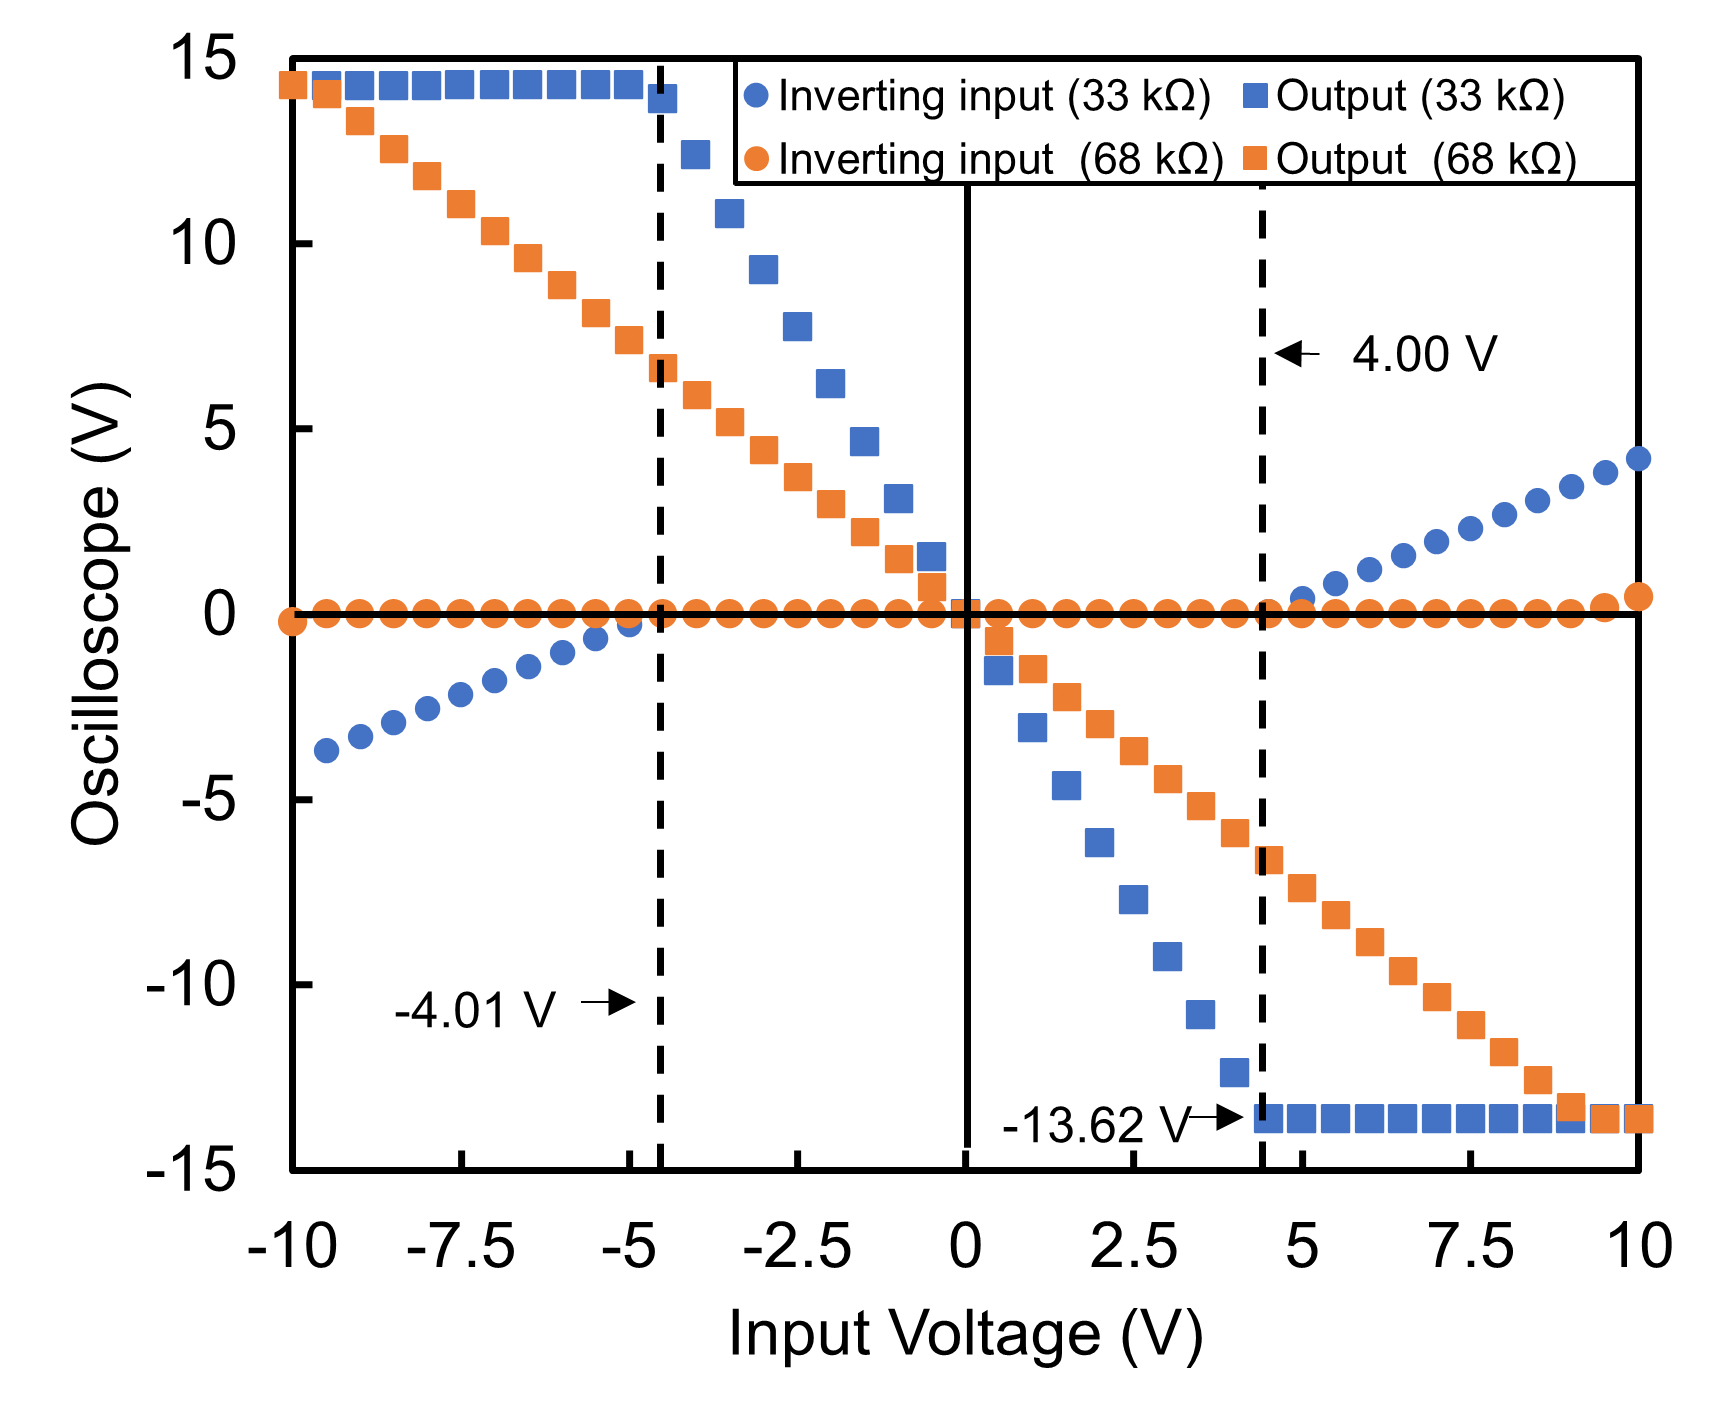
\includegraphics[width=0.94\columnwidth]{fig1.JPG}
% \end{figure}

\end{document}